%  +---------------------------------+
%  | LaTeX template file for AES LAC |
%  +---------------------------------+
% This file is a modification of the template used for the
% AES Brazil.
% To be used with "aeslac.cls" version 1.0

%%
%% NOTE: This text file uses UNIX line feed conventions. When (human)
%% reading this file on other platforms, you may have to use a text
%% editor that can handle lines terminated by the UNIX line feed
%% character (0x0A).
%%

%%%%%%%%%%%%%%%%%%%%%%%%%%%%%%%%%%%%%%%%%%%%%%%%%%%%%%%%%%%
%
%  CARGADO DE LA CLASE
%
% La clase "aeslac.cls" carga automáticamente los siguientes paquetes:
%    hyperref, graphicx, color, times, y helvet.
% El paquete "graphicx.sty" es necesario para incluir imágenes,
% gráficos, etc. El uso de pdflatex requiere que el formato de las
% imágenes sea PDF, PNG, o JPG (no EPS).

% Para generar el documento en formato DVI, eliminar la opción 'pdfout'
% y ejecutar
% > latex template
% > bibtex template
% > latex template
%
% Para generar el documento en formato PDF ejecutar:
% > pdflatex template
% > bibtex template
% > pdflatex template

% Eliminar la opción "pdfout" si no se está usando 'pdflatex'.
% La opción "ams" carga los paquetes "amsmath", "amssymb" and "amsthm".
\documentclass
  [ams,pdfout]% opciones de la clase
	{aeslac}

%%%%%%%%%%%%%%%%%%%%%%%%%%%%%%%%%%%%%%%%%%%%%%%%%%%%%%%%%%%
%
% CARGADO DE PAQUETES
%
% Usar \RequirePackage en lugar de \usepackage
% Esto evita conflictos entre paquetes.

% Usar formato 8-bit UCS/Unicode Transformation Format
\RequirePackage[utf8]{inputenc}

% Para escribir el documento en español es necesario usar la opción
% "spanish" de "babel"
\RequirePackage[spanish]{babel}

% Usar caracteres extendidos
% Solo es necesario para escribir en portugués
\RequirePackage{textcomp}

%\let\oldcdot\cdot
%\usepackage{breqn}
%\let\cdot\oldcdot

\DeclareMathOperator*{\argmin}{argmin}

\begin{document}
% La página del título es construida en el ambiente "TitlePage".
% En ese ambiente se genera el título, los autores y
% sus respectivas afiliaciones y el resumen, en ese orden.
\begin{TitlePage}
	% El titulo es producido con el comando \Title.
	\Title{Alineación audio-partitura para música ejecutada con flauta traversa}
	% \RunningTitle y \RunningAuthors son impresos en el
	% encabezado de cada página.
	\RunningTitle{Alineación audio partitura en la flauta traversa} % titulo corto
	% 2 o mas autores:
	% ("Autor1 y Autor2" para 2 autores.)
	% ("Autor1 et al." para 3 o mas autores.)
	\RunningAuthors{Juan P. Braga Brum et al.}
% Especificar autor y afiliación (con \Author y \Affil) para cada
% autor (en ese orden).
% Primer autor
	\Author
		[juanbragabrum@gmail.com]% email
		{Juan P. Braga Brum} % Nombre del autor (impreso en la página del titulo)
		\Affil
			[A]% clave (argumento opcional)
			{%
				Universidad de la República (UdelaR),
				Facultad de Ingeniería (FIng),
				Instituto de Ingeniería Eléctrica (IIE)\\
				Montevideo, 11300, Uruguay
			}
	\Author
		[wagner@smt.ufrj.br]
		{L. W. P. Biscainho}
		\Affil
			[B]% clave (argumento opcional)
			{%
				Universidade Federal do Rio de Janeiro (UFRJ), 
				Escola Politécnica (Poli),
				Departamento de Engenharia Eletrônica e de Computação (DEL)\\
				Rio de Janeiro, RJ, 21941-972, Brasil
}
	\Author
		[pcancela@fing.edu.uy]
		{Pablo Cancela}
		\Affilref[A]
	
	\Abstract{%
		El problema de alineación entre audio y partitura para música ejecutada con flauta traversa es abordado en la presente publicación. Con ese fin se hace un estudio del estado del arte en el área, así como un abordaje musicológico desde las técnicas de ejecución del instrumento. Se plantea una solución al problema para señales de flauta ejecutadas con técnicas tradicionales y la evaluación cuantitativa de desempeño en una base de datos desarrollada con este propósito. Se plantean los desafíos que presenta el repertorio contemporáneo ejecutado con técnicas extendidas. Además, la base de datos se hace disponible para futuros trabajos en el área con fines académicos. 
		 
		%
	}%
\end{TitlePage}
%
% Los títulos de las secciones se escriben usando mayúsculas
\section{Introducción}

La alineación entre audio y partitura es la asociación entre dos tipos de datos: muestras de audio digital y notación simbólica de música. Es un tema de investigación que ha captado la atención durante más de 30 años, de la comunidad científica en áreas como el Procesamiento de Audio, Machine Learning y Computer Music \cite{orio2003score}. El problema se puede dividir en dos grandes enfoques de resolución en \textit{online}\footnote{Refiere a análisis en tiempo real} y \textit{offline}, cada uno con aplicaciones diferentes y características propias de la estrategia utilizada.

%
El enfoque offline cuenta con toda la interpretación de la obra mediante un archivo de audio al momento de procesamiento, siendo posible analizar de forma no causal y lograr mayor precisión en la alineación partitura y audio. Se puede ver como el indexado de las muestras de audio según la información de la partitura. En otras palabras, asociar los eventos simbolizados en la partitura con las correspondientes muestras de audio de una grabación, como se esquematiza en la Figura \ref{fig:resultado_alineacion}. La resolución del problema offline tiene diversas aplicaciones de interés como los editores de audio inteligentes que acceden al audio a través de compases y notas de la partitura, búsquedas asistidas en grandes bases de datos a partir de fragmentos de notación musical, herramientas para el análisis automático de parámetros expresivos como son las dinámicas, variaciones de tempo, articulaciones, entre otros \cite{dannenberg2006music}.

\begin{figure}[h!]
\begin{center}
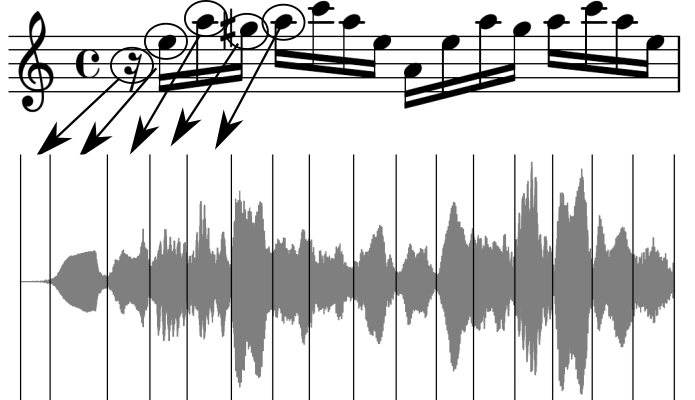
\includegraphics[width=0.4\textwidth]{imagenes/resultado_alineacion} 
\caption{Esquema conceptual del problema de alineación audio y partitura.}
\label{fig:resultado_alineacion}
\end{center}
\end{figure} 

%
En cambio, la resolución del problema en tiempo real cuenta con la información disponible a cada instante, determinando la alineación de forma causal únicamente con datos del pasado. Tiene como principal motivación transformar la interacción entre computadora-humano en una experiencia bidireccional, simulando el comportamiento de una interpretación de un músico con otro. Denominado también como acompañamiento automático o músico sintético\cite{vercoe1984synthetic} fue la motivación que dió comienzo a esta línea de investigación. Otras aplicaciones como un pasador de páginas automático\cite{arzt2008score}, o el despliegue de información sincronizada en un concierto de orquesta\cite{prockup2013orchestral} han sido presentadas recientemente.  

%
Por otro lado, la flauta traversa es elegida por muchos compositores en la practica compositiva. En particular, para la creación de música electroacústica para medios mixtos\footnote{Música donde se combina el material sonoro generado por una computadora con la ejecución de instrumentos musicales.}. Es claro que esta corriente musical se ve favorecida por aplicaciones basadas en algoritmos de alineación audio partitura, motivación detrás del presente trabajo que acota el problema a música ejecutada con flauta traversa. Dando lugar a la creación de una base de datos compilada a partir de obras de referencia del repertorio de la flauta, que se hace pública para su uso con fines académicos.

%
\section{Alineación audio-partitura}

La resolución del problema de alineación entre audio y partitura es generalmente dividida en dos etapas. En primer lugar, ambas representaciones de la misma pieza musical (i.e. grabación y notación simbólica) son transformadas a un espacio de características donde puedan ser comparables matemáticamente, usualmente llamado como representación intermedia. Ésta transformación genera a la salida dos series temporales de vectores con los que se determina la correspondencia punto a punto mediante algún algoritmo de alineación.

El enfoque de resolución que se implementa en el presente trabajo esta basado en \textit{Dynamic Time Warping (DTW)} debido a que los mayores desempeños reportados en los últimos 10 años lo utilizan (ver tabla \ref{tab:Mirex} resumen de la competencia MIREX\footnote{http://www.music-ir.org/mirex/wiki/MIREX\_HOME} en alineación audio partitura en tiempo real). Ésta técnica además, se ha aplicado con éxito en la resolución de problemas de \textit{Speech Recognition}. Por este motivo se dejan de lado enfoques estadísticos de resolución del problema, donde se destaca por ser el enfoque más extendido basado en HMM (de su denominación en inglés \textit{Hidden Markov Models}) y se deja de lado. Para más información se recomienda dirigirse a las publicaciones \cite{montecchio2009discrete,raphael1999automatic,orio2001score}. 


\subsection{Dynamic Time Warping}

Para la definición del problema de alineación de forma matemática, supóngase que se tienen dos series temporales $\vec{X}\in\mathbb{R}^{M\times D}$ y $\vec{Y}\in\mathbb{R}^{N\times D}$, donde $D$ es la dimensión del vector de características, y $M$ y $N$ el largo de las mismas respectivamente. La alineación está dada por dos secuencias, dígase $p, q \in \mathbb{N}^{L}$, que definen la correspondencia punto a punto entre $\vec{X}$ e $\vec{Y}$. Por lo que, de forma matemática se dice que $\vec{X}[p[i]]$ y $\vec{Y}[q[i]]$ están alineados. Para encontrar la correspondencia entre series se debe resolver el siguiente problema de minimización:

\begin{equation}
p,q = \argmin_{p,q} \sum_{i=1}^{L} d(\vec{X}[p[i]],\vec{Y}[q[i]]) 
\end{equation}

Este problema de minimización, con algunas restricciones sobre las secuencias $p$ y $q$, es resolube con el algoritmo denominado como DTW (\textit{Dynamic Time Warping} por su denominación en inglés). Esta es una técnica consolidada para la alineación de series numéricas con fuerte correspondencia temporal. 

El primer paso es el cómputo de $D$ la matriz de similaridad, que depende estrictamente de la distancia utilizada, el cálculo se define matemáticamente como
\begin{equation}
\label{eq:matrizsimilaridad}
D[i,j] = d(\vec{X}[i],\vec{Y}[j])
\end{equation}
donde $D[i,j]$ tiene $M\times N$ elementos donde representan la distancia entre todos los pares de puntos de las series temporales $\vec{X}$ e $\vec{Y}$.  


El segundo paso corresponde al computo de $C$ la matriz de costo acumulada. El cálculo se hace de forma recursiva como muestra la siguiente ecuación (esta no es la única forma de calcular la matriz de costo como se verá más adelante), 

\begin{equation}
\label{eq:matrizcosto}
C[i,j] = min\left\lbrace  
\begin{array}{ll}
C[i,j-1] + w_h\cdot D[i,j]\\
C[i-1,j] + w_v\cdot D[i,j]\\
C[i-1,j-1] + w_d\cdot D[i,j]
\end{array}
\right.
\end{equation}
donde $C[i,j]$ es el costo del camino menos costoso, desde el punto $(1,1)$ hasta el $(i,j)$. Además $C[1,1]=d(\vec{X}[1],\vec{Y}[1])$. Los valores $\vec{w}=(w_h,w_v,w_d)$\footnote{Notar que los subindices refieren respectivamente a dirección horizontal, vertical y diagonal} son factores de penalización, donde valores mayores que $1$ desalientan movimientos en la dirección correspondiente. A efectos de los cálculos en la presente tesis, siguiendo las recomendaciones de \cite{sakoe1978dynamic}, se utiliza $\vec{w}=(1,1,2)$ para no penalizar ninguna dirección. 

Luego que se completa el cómputo de la matriz $C$, se busca el camino de menor costo obteniendo la alineación entre series dada por $p$ y $q$. Éste se encuentra haciendo recursión hacia atrás desde $C[M,N]$ hasta $C[1,1]$. El algoritmo se compone de decisiones locales óptimas bajo el supuesto de que el resultado será un mínimo global. En concreto, se comineza desde $C[M,N]$ evaluando todas las celdas vecinas buscando el mínimo, éste se agrega al comienzo del camino y de forma sucesiva el procediemitno finaliza al llegar a $C[1,1]$.


Por otro lado en las ecuaciones \ref{eq:dist_coseno_ok} y \ref{eq:dist_euclideana} se definen de forma matemática dos distancias de uso común en la literatura para la resolución del problema y las usadas en los experiemntos.


\begin{equation}
\label{eq:dist_coseno_ok}
d_{coseno}(\vec{X},\vec{Y}) = 1 - \frac{\vec{X}\cdot\vec{Y}}{\lVert\vec{X}\rVert_{2}\lVert\vec{Y}\rVert_{2}}
\end{equation}

\begin{equation}
\label{eq:dist_euclideana}
d_{euclideana}(\vec{X},\vec{Y}) = \lVert \vec{X} - \vec{Y} \rVert_{2}
\end{equation}


\subsection{Restricciones}
\label{sec:restricciones}

Las restricciones sobre el camino acotan el universo de posibilidades en la búsqueda del mínimo, disminuyendo el costo computacional en el cálculo de la alineación. La elección correcta de estas restricciones está asociada al conocimiento a priori del problema que se quiera resolver, es así que se pueden aplicar sin atentar contra el resultado final. En lo que sigue se hará mención solamente de las restricciones que fueron aplicadas para los experimentos de la tesis, para más detalle se recomienda el libro de M. Muller \cite{muller2007information}.
  
En el caso partícular de alineación entre audio y partitura existe una correspondencia directa entre notación simbólica y las grabaciones de audio. Es claro si se tiene en cuenta que el músico ejecuta la pieza mediante la lectura de la partitura. Ésta característica de las series temporales en el problema planteado, permiten aplicar las restricciones que se especifican a continuación:

\begin{itemize}
\item \textbf{Limites}: Los limites de la alineación deben cumplir la siguiente condición: $p[1] = q [1] = 0$ y $p[L] = M, q[L] = N$. Es razonable suponer que la grabación empieza y termina con la ejecución del cominezo y el final de la partitura.
\item \textbf{Monotonicidad}: Las secuencias deben cumplir: $p[i+1] \geq p[i]$ y $q[i+1] \geq q[i]$. Teniendo en cuenta que la ejecución de la partitura se hace en una lectura direccionada (i.e. de izquierda a derecha) sin cambios a la dirección contraria parece una restricción acorde. 
\item \textbf{Continuidad}: Por último se impone: $p[i+1] \leq p[i] + 1$ y $q[i+1] \leq q[i] + 1$.  Suponiendo que el intérprete no realiza ningún salto en la lectura de la partitura durante la ejecución no debería resultar en el descarte de una solución válida. 
\end{itemize}


\subsection{Estado del arte}

Existen diversas implementaciones de sistemas de alineación audio partitura con DTW, en la publicación \cite{orio2001alignment} una estructura espectral de picos es generada a partir de la partitura y es utilizada para el cálculo de distancia con las ventanas de audio analizadas. Aseguran que esta metodología es aplicable a señales polifónicas logrando mejores resultados y mayor robustez que las técnicas basada en extracción de pitch. Por otro lado en \cite{dannenberg2006music} se propone la utilización de DTW con extracción de características basadas en la representación tiempo frecuencia denominada como Chromagrama, este mismo sistema es presentado para la resolución del problema de \textit{Music Retrieval} en grandes bases de datos. Dixon en la publicación \cite{dixon2005live} es el primero en proponer una variante de DTW para la resolución del problema en tiempo real con la información disponible a cada instante, sacrificando el desempeño del algoritmo. Además, en \cite{gagnon2007high} el camino optimo de alineación es calculado a partir de información de alto nivel como es chroma y una estimación de la duración y ritmo local a partir de la señal de análisis. 

\begin{table}[!ht]
\caption{Resultados de la competencia Mirex en Real-time  Audio to Score Alignment.}
\label{tab:Mirex}
\vspace*{10pt}
\centering
\small
\begin{tabular}{ll}
\textbf{Autor (Año)}	&	\textbf{Resultado}\\ \hline
Francisco J. Bris Peñalver (2017)     & 94\%   \\
Francisco J. Rodriguez Serrano (2016) & 97\%   \\
Francisco J. Rodriguez Serrano (2015) & 95\%   \\
Chunta Chen* (2014)                   & 91\%   \\
Julio J. Carabias Orti (2013)         & 86\%   \\
Julio J. Carabias Orti (2012)         & 83\%   \\
Kosuke Suzuki (2011)                  & 67\%   \\
\textit{*Con un algoritmo offline}
\end{tabular}
\end{table}


Un salto cualitativo en los resultados del MIREX (observar tabla \ref{tab:Mirex}) fue logrado por el algoritmo implemetado por J. Carbias y detallado en la publicación\cite{carabias2015audio}. El sistema está separado en dos etapas: una etapa de procesamiento y a continuación la de alineación. En la primera etapa se hace la síntesis de la notación simbólica y mediante el análisis se obtienen patrones espectrales asociados a cada unidad de la partitura. Estos son aprendidos desde el audio generado por la síntesis, mediante la factorización espectral basada en NMF (\textit{Non-Negative Matrix Factorization} por su denominación en inglés). En la segunda etapa la descomposición espectral de la magnitud del espectrograma es realizada con los patrones aprendidos previamente resultando en una matriz de distorsión, que es utilizada como matriz de costo para el cómputo de DTW de forma online. La alternativa presentada por FJ Rodriguez Serrano\cite{rodriguez2017tempo}, que actualmente tiene el mejor resultado en la competencia, define el estado del arte. El algoritmo esta basado en el de J. Carabias donde el cómputo de la alineacíon se hace con DTW incorprorando información del tempo de la interpretación, mejorando notoriamente los resultados.

%
\section{Flauta traversa}

La naturaleza sonora 
Las técnicas para la ejecución del instrumento se pueden dividir en dos grandes grupos. Por un lado existen las denominadas técnicas tradicionales, de uso común del instrumento, asociadas a la generación de música principalmente basada en alturas y duraciones. Por otro lado, los compositores y flautistas contemporáneos han definido las llamadas técnicas extendidas\footnote{El desarrollo de técnicas extendidas tiene estrecha relación con el desarrollo de la música electroacústica. La síntesis electrónica y la manipulación electroacústica del sonido introdujeron nuevas sonoridades, que suministraron modelos para la experimentación en la música instrumental}. Éstas, como su nombre lo indica, extienden las capacidades sónicas del instrumento generando material sonoro que va más allá del definido con alturas y duraciones.

%
\subsection{Técnicas tradicionales}

Las técnicas tradicionales de la flauta son aquellas con las cuales el material sonoro ejecutado es definible mediante los parámetros de altura y duración. Como su nombre lo indica, las mismas refieren al uso tradicional de la flauta traversa y sus mecanismos de producción de sonido. Para comprender la naturaleza de las señales generadas con técnicas tradicionales es necesario identificar por un lado la producción de la excitación periódica, y en complemento a lo anterior el largo de la columna de aire. 

%
\subsection*{Producción del sonido}

Para poner en oscilación al instrumento, el flautista debe soplar superando en el interior de su boca la presión atmosférica. Las ondas oscilatorias son generadas a partir de la colisión del flujo de aire con el filo del agujero de la embocadura. En otras palabras, la turbulencia provocada por la colisión genera una onda viajera que se traslada a través del flujo de aire. Ésta es la que pone a resonar la columna de aire interior al tubo de la flauta. De esta forma, se genera un sonido de naturaleza periódica denominado como nota musical. En complemento, la frecuencia fundamental de la nota emitida depende estrictamente del largo de la columna de aire. Para el control de este parámetro, existen las llaves del instrumento (en la flauta moderna) que tapan o liberan los agujeros del tubo. Un agujero libre significa la imposición de presión atmosférica en ese punto de la columna de aire, definiendo de esta forma el largo de la misma.

%
\subsection*{Modos de Vibración}

En la práctica, una configuración de llaves en el instrumento permite más de un modo de vibración\footnote{Refiere a las ondas estacionarias que un medio de propagación y sus características permiten.}, generando otras alturas musicales que se suman a la de frecuencia fundamental. Se tiene entonces, que para una columna de aire con largo determinado (i.e. posición de llaves determinada por el instrumentista) resonando en el interior del tubo, existe emisión simultánea de otras alturas musicales por encima de la de frecuencia fundamental. Éstas dan un sonido característico y se las denomina armónicos. 

%
De forma teórica se pueden deducir los armónicos permitidos por la construcción del instrumento, modelándolo como un tubo cilíndrico con sus dos extremos abiertos. De lo anterior, se deduce que la onda de mayor longitud que soporta las condiciones de borde\footnote{Las condiciones de borde refiere a la imposición de nodos de presión en los extremos del tubo cilíndrico.} tiene una longitud de dos veces la distancia entre los nodos de presión (en su forma matemática se escribe como $\lambda=2L$). De la misma forma, se deduce que existen otras longitudes de onda permitidas en este modelo, y se demuestra matemáticamente que cumplen $\lambda=2L/k$, con $k \in N$.

%
Por otro lado, la frecuencia del modo de vibración se calcula como la velocidad de propagación de la onda sobre la longitud de la misma, matemáticamente se expresa como $f=v/\lambda$. De la relación anterior se deduce en primer lugar, que la mayor longitud de onda provoca la altura más baja, que en el caso particular de la flauta es la frecuencia fundamental. En segundo lugar, que la estructura armónica de la flauta se puede expresar como $f_{i}=(i+1)f_{0}$, donde $i \in N$ y $f_{0}$ es la frecuencia fundamental en Hertz. 

%
\subsection*{Registro}

Esta característica asociada al instrumento determina el rango de frecuencias emitibles en el instrumento. La cota inferior del registro queda determinada por el pie elegido, para el caso de \textit{pie en $C$} el limite es el $C4$, por el contrario para \textit{pie en $B$} es el $B3$. Del otro lado, en la parte alta del registro, la flauta moderna alcanza notas superiores a $C7$, en particular $C\#7$ y $D7$ (observar Figura \ref{fig:registro_flauta}). La producción del sonido a partir de $A6$ se vuelve dificultosa, siendo posible para flautistas expertos \cite{samuel2002study}.

\begin{figure}[h!]
\begin{center}
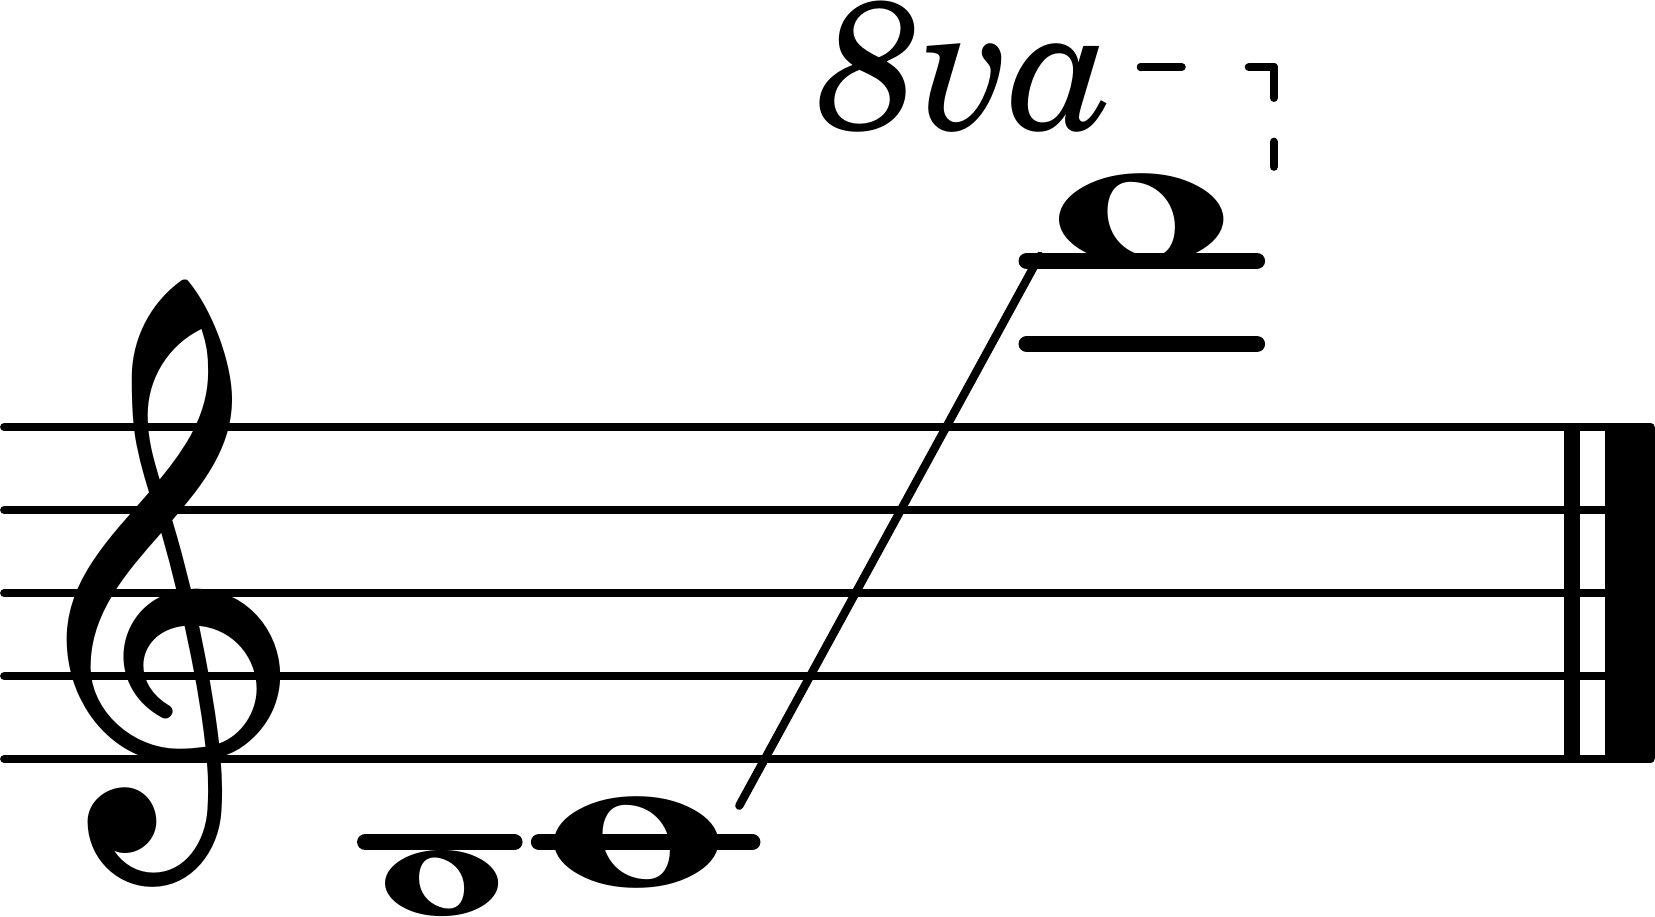
\includegraphics[width=0.15\textwidth]{imagenes/registro_flauta} 
\caption{Registro de la flauta traversa. Se observa la cota inferior del registro para flauta con \textit{pie en $B$} y \textit{pie en $C$}.}
\label{fig:registro_flauta}
\end{center}
\end{figure} 

%
\subsection{Técnicas extendidas}

No es objetivo de esta sección hacer una descripción exhaustiva del material sonoro generado con las distintas técnicas, para eso existe extensa bibliografía \cite{samuel2002study,dick1975other}. Por el contrario, presentar los aspectos relevantes para la comprensión de la naturaleza de las señales de flauta, y los desafíos que presentan las técnicas extendidas en áreas científicas de investigación con el \textit{Music Information Retrieval} (por su denominación en inglés).   

%
Con el afán de extender el lenguaje musical, los compositores contemporáneos\footnote{E.g. George Crumb (Estados Unidos, 1929), Helmut Lachenmann (Alemania 1935), Salvatore Sciarrino (Italia, 1947).} se han dedicado a explorar las capacidades sónicas de los instrumentos musicales. Para esto, se siguen procedimientos como la intervención\footnote{Denominado también como la preparación de instrumentos. Por ejemplo, el piano preparado de John Cage (Estados Unidos, 1912-1992) y la cabeza móvil en la flauta traversa (\textit{Glissando Headjoint} por su denominación original) de Robert Dick (Estados Unidos, 1950).} mecánica de instrumentos o la definición métodos no ortodoxos de ejecución. Es así, que en el caso particular de la flauta se ha derribado el mito de que la sonoridad del instrumento es limitada, y hoy en día existe un diccionario bien definido de técnicas reproducibles, denominadas extendidas\cite{dick1975other}. Algunas de las técnicas más conocidas se enlistan a continuación (se utilizan las denominaciones en inglés):

\begin{itemize}

\item \textbf{Flutter Tonguing:} Refiere a la generación del soplido con aleteo de la lengua. 
\item \textbf{Tongue Noises:} Ruidos con la lengua dentro de la embocadura. 
\item \textbf{Percussive Sounds:} Presión de las llaves de forma percusiva.
\item \textbf{Microtonal Inflections:} Inflecciones microtonales.
\item \textbf{Multiphonics:} Sonidos multifónicos (más de una nota a la vez con el instrumento).
\item \textbf{Cantar y tocar a la vez:} Como su nombre lo hace explicito la ejecución de dos alturas a la vez mediante el canto y el instrumento.

\end{itemize}

%
La exploración en la música contemporánea abarca también el control tímbrico y la calidad del sonido como un parámetro notado por el compositor. En esta línea, la ejecución de sonidos de banda angosta y banda ancha son muchas veces elementos buscados desde la composición. En el caso particular de la flauta, este nuevo material sonoro se ejecuta mediante el control de la embocadura\footnote{El término embocadura refiere al aparato de producción de la excitación de la columna de aire, en conjunto con la técnica de soplido.} así como la presión de aire. Para la alineación entre audio y partitura en este tipo de obras no es suficiente con la representación basada en alturas y duraciones, a diferencia de lo que sucede con el lenguaje tradicional de la flauta. Se vuelve necesario entonces explorar otras representaciones intermedias de las basadas en la escala cromática (i.e. CQT y Chromagrama) para la resolución del problema de alineación entre audio y partitura en obras del repertorio contemporáneo.      

\subsection{Alcance y desarrollo de la publicacion}
%

%



\section{Metodología}

En la Figura \ref{fig:diagrama_general} se esquematiza la método de resolución abordado. Por un lado, el bloque de extracción de contenido musical tiene el objetivo de transformar muestras de audio en representación intermedia. Del otro lado, el bloque de codificación de notación simbólica, lleva la partitura a la misma representación. 

Dado que las señales de flauta de la base de datos son ejecutadas con técnicas tradicionales el material sonoro se encuentra organizado en alturas de la escala cromática de 12 tonos (también llamada como la escala de música occidental). Estos sonidos, por su naturaleza se organizan dos formas: por alturas absolutas o por clases de altura. Es por eso que para la extracción de contenido musical se opta respectivamente por la \textit{Constant Q Transform}\cite{schorkhuber2010constant} (CQT) y el \textit{Chromagrama} (computado a partir del cálculo de la CQT).

\begin{figure}[h!]
\begin{center}
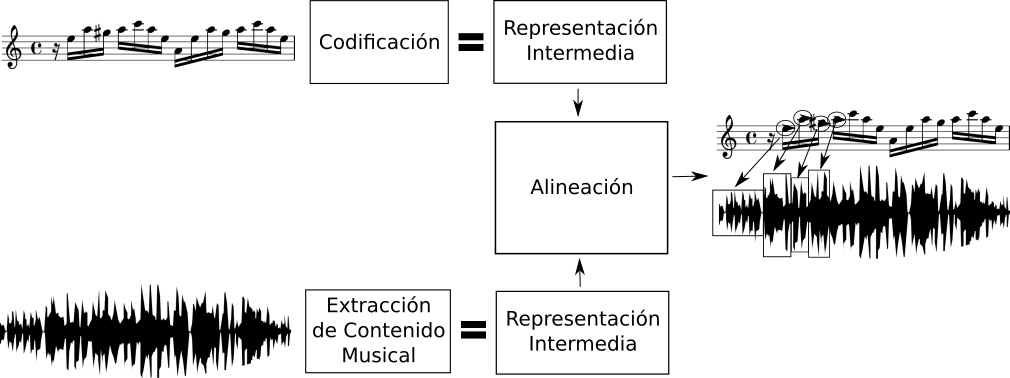
\includegraphics[width=0.5\textwidth]{imagenes/diagrama_general-back} 	
\caption{Esquema general de la solución del problema de alineación entre audio y partitura utilizada en el presente trabajo.}
\label{fig:diagrama_general}
\end{center}
\end{figure}

\subsection{Extracción de contenido musical}
La escala de la música occidental tiene 12 sonidos por octava, donde las frecuencias fundamentales se ditribuyen de forma geométricamente espaciada. Suponiendo afinación éstandar de $440Hz$ matemáticamente se escribe como:
\begin{equation}
\label{eq:escalaTI}
F_k= 440Hz \times 2^{\:k/12} \: \text{con} \: k \: \in \: [-50,40]
\end{equation}

Como se detalla en la publicación \cite{brown1991calculation} la representación espectral CQT fue diseñada con el propósito de adaptarse a la organización en alturas de los sonidos musicales. Puede ser directamente calculada mediante una evaluación conveniente de la DFT. El \textit{k-ésimo} componente se escribe como: 
\begin{equation}
\label{eq:CQT}
X^{CQT}[k]=\frac{1}{N[k]}\sum_{n=0}^{N[k]-1}w[n,k]x[n]e^{-j2\pi Qn/N[k]}
\end{equation}
donde el factor de normalización $1/N[k]$ aparece para compensar la dependencia con $k$ del número de términos en la sumatoria. Para el problema que aquí se quiere resolver, la mínima resolución queda determinada por la cantidad de semitonos en la escala cromática. Es así que como mínimo se trabaja con 12 bins por octava. Por otro lado, para analizar todo el espectro es necesario que $\Delta_{f_k}=f_{k+1}-f_{k}=f_k(2^{\frac{1}{B}}-1)$ por lo que con $B=12$ se cumple que $Q=1/(2^{\frac{1}{12}}-1)\approx 17$. De esta forma queda determinado el tamaño de las ventanas de análisis de la CQT en función de la cantidad de Bins por octava, siendo este parámetro el que define el compromiso tiempo frecuencia de la transformada. 
 
El cálculo de la CQT se hace en el rango de frecuencias: $B3$ a $B8$. Con el criterio de abarcar el registro más amplio posible, teniendo en cuenta por un lado el límite inferior del registro de la flaut, y por otro, que las señales están muestreadas a $44100Hz$. Además, teniendo en cuenta que el Chromagrama se cálcula colapsado la CQT se calcula en octavas completas. Por lo que se obtiene para la CQT un vector de dimensión 72 y para el Chromagrama de 12.

\subsection{Codificación de la partitura}

El bloque de codificación tiene como entrada notación simbólica y a la salida genera una matriz que codifica en el eje vertical las alturas mientras que en el horizontal las duraciones (de forma análoga a la CQT y Chromagrama). La hipotesis central radica en el modelado de la notación exclusivamente bajo los parámetros de altura y duración, dejando de lado las dinámicas, articulaciónes y otros parámetros expresivos. 

La duración en notación musical es expresada de forma relativa a la redonda. Para obtener la duración entonces se debe tener en cuenta el tempo sugerido por el compositor, de esta forma transformar un valor relativo de la redonda a segundos.  

Por otro lado, la posición en el eje vertical queda determinada por la altura musical notada. Para esto se tienen en cuenta dos aspectos independientes, por un lado la forma de representar las alturas musicales (específicamente como alturas absolutas o clases de altura) y por otro lado la cantidad de \textit{bins} (parámetro del sistema) que completan una octava musical. Además, la intensidad es codificada con el valor unidad (se trabaja con valores normalizados). Esta decisión se desprende del hecho que las dinámicas no se tienen en cuenta para la codificación. 

Dos aspectos importantes se tienen encuenta para la codificación de la partitura. Por un lado la representación de los silencios musicales y la cántidad de armónicos en los momentos de notas. El primero se representa como un valor constante $\beta$ en todo el registro. Del otro lado, en función de la naturaleza sonora de la flauta los armónicos. La decisión de los mejores parámetros es determinada en función de los resultados con la base de datos y se verá mas adelante. En la Figura \ref{fig:armonicos_param} se observa la varición en el resultado según la cantidad de armónicos.

\begin{figure}[h!]
\begin{center}
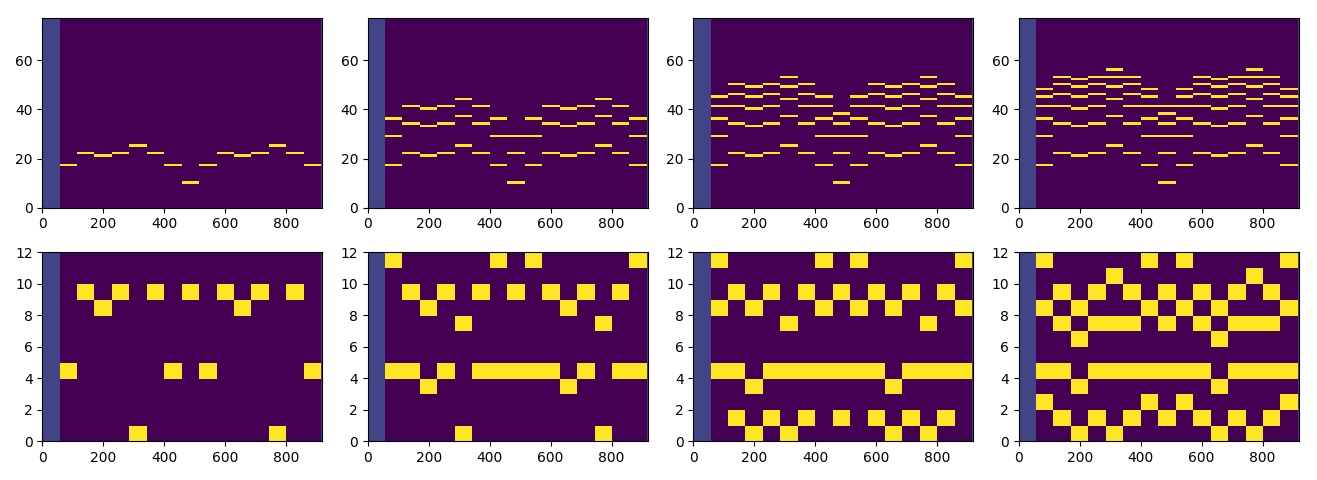
\includegraphics[width=0.48\textwidth]{imagenes/armonicos_param} 	
\caption{Cantidad de armónicos en la codificación. Arriba en alturas absolutas, abajo en clases de altura. De izquierda a derecha los armónicos elegidos son 0, 2, 4 y 6. Generado con el primer compás del movimiento Allemande de BWV 1013 de J.S. Bach.}
\label{fig:armonicos_param}
\end{center}
\end{figure}

\section{Experimentos}

La sección esta dividida en tres partes. Se comienza evaluando la influencia de los parámetros de representación intermedia en el resultado de alineación para determinar la mejor combinación. Posteriormente, se evalúan distintas restricciones en el cámino óptimo de alineación de DTW. Luego, se hace una comparación de la estrategia de codificación de notación simbólica propuesta aquí, frente a la síntesis como paso intermedio. Para finalizar se hace una comparación con un algoritmo desarrollado por terceros. Todos los experimentos son realizados en el presente capítulo se realizan con la base de datos construída en el marco de la tesis. 

\subsection{Medidas de desempeño}
\label{sec:medidas_desempeno}

Para la evaluación de desempeño como se recomienda en la publicación \cite{orio2003score} se utilizan dos medidas, la tasa de aciertos y la precisión\footnote{Definida en este caso como una medida de desfasaje temporal entre las anotaciones y el resultado de la alineación.}. La primera cuantifíca la cantidad de notas bien identificadas, como porcentaje del total. Por otro lado, la precisión es el promedio del desfasaje de las notas bien identificadas con respecto al ground truth.

A la salida de la etapa de alineación se obtiene una lista como la representada en la Figura \ref{fig:datos_tabla}. Ésta es comparada con el ground truth correspondiente. Siendo $u(t_u)$ la altura del resultado de la alineación (i.e. frecuencia representada en midi) y $v(t_v)$ la del ground truth, en los tiempos $t_v$ y $t_u$ respectivamente, se definen los aciertos como los puntos que cumplen $|t_v-t_u|<tol$, si $u(t_u)=v(t_v)$. Por otro lado, la precisión matemáticamente se define como $\frac{\sum{|t_u-t_v|}}{N}$ siendo $N$ el largo de $v$ (i.e. la cantidad de notas en el ground truth). Para los cálculos del presente capítulo se definió la tolerancia $tol=200ms$ como se sugiere en la publicación \cite{orio2001alignment}.

\begin{figure}[h!]
\begin{center}
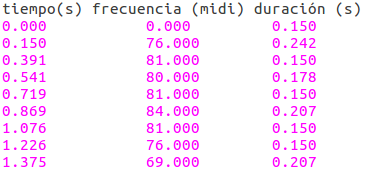
\includegraphics[width=0.4\textwidth]{imagenes/datos} 	
\caption{Ejemplo del resultado de etapa de alineación. Se observa la serie temporal representada como comienzo, altura y duración de las notas musicales.}
\label{fig:datos_tabla}
\end{center}
\end{figure}

\subsection{Base de datos de flauta tradicional}

La flauta traversa cuenta con un repertorio vasto de obras musicales asociado a su larga historia,  diversos compositores han compuesto para este instrumento. La base de datos esta compuesta por fragmentos de cuatro piezas musicales ejecutadas con técnicas tradicionales. La elección de las obras determina variaciones sustanciales en los estilos musicales que la componen. Las obras seleccionadas son:
\begin{itemize}
\item Allemande, BWV 1013 de J.S. Bach
\item Syrinx de C. Debussy
\item Density 21.5 de E. Varese
\item Sequenza I de L. Berio
\end{itemize} 

%
De las cuatro obras musicales se tomaron grabaciones de distintos intérpretes para lograr variación en aspectos expresivos. De estas grabaciones se generaron fragmentos de forma que la unidad mínima fuere una frase musical\footnote{La frase musical es una de las unidades más pequeñas en una composición musical. Esta asociada a la sensación de completitud (inicio, desarrollo y fin) de una idea musical, similar a la idea de frase en la composición literaria. En el caso particular de la flauta traversa, esta generalmente asociada a la sección de música entre respiración y respiración\cite{blom1955grove}.} y genearon archivos de anotaciones manuales como ground truth. Resultando en un total de 30 fragmentos de audio con un archivo de texto con notación simbólica y con anotaciones manuales. Las notas que aparecen en la base van desde $C4$ a $D7$. En total existen $2245$ eventos, entre notas y silencios. La base se encuentra accesible para su uso con fines académicos en: https://www.kaggle.com/jbraga/traditional-flute-dataset.


\begin{table}[!ht]
\caption{Tabla con el detalle de los rangos de valores considerados para el ajuste de parámetros.}
\label{tab:parametros}
\vspace*{10pt}
\centering
\small
\begin{tabular}{ll}
\textbf{Parámetro}	&	\textbf{Valores}\\ \hline
Organización           & Alturas Absolutas - Clases de Altura        \\ 
Resolución ($ms$) & 1.4 - 2.9 - 5.8 - 11.6 - 23.2 - 46.4        \\ 
Bins por octava                       & 12 - 24 - 36                                \\ 
Armónicos                             & 0 - 1 - 2 - 3 - 4 - 5 - 6                   \\ 
$\beta$ (Beta)                        & 0.1 - 0.4 - 0.7 - 1.0  \\ 
\end{tabular}
\end{table}

\subsection{Ajuste de parámetros representación intermedia}
En lo que sigue se presenta el ajuste de parámetros de representación intermedia. Para eso se compara el desempeño con los parámetros de la  tabla \ref{tab:parametros}.

\begin{figure}[h!]
\begin{center}
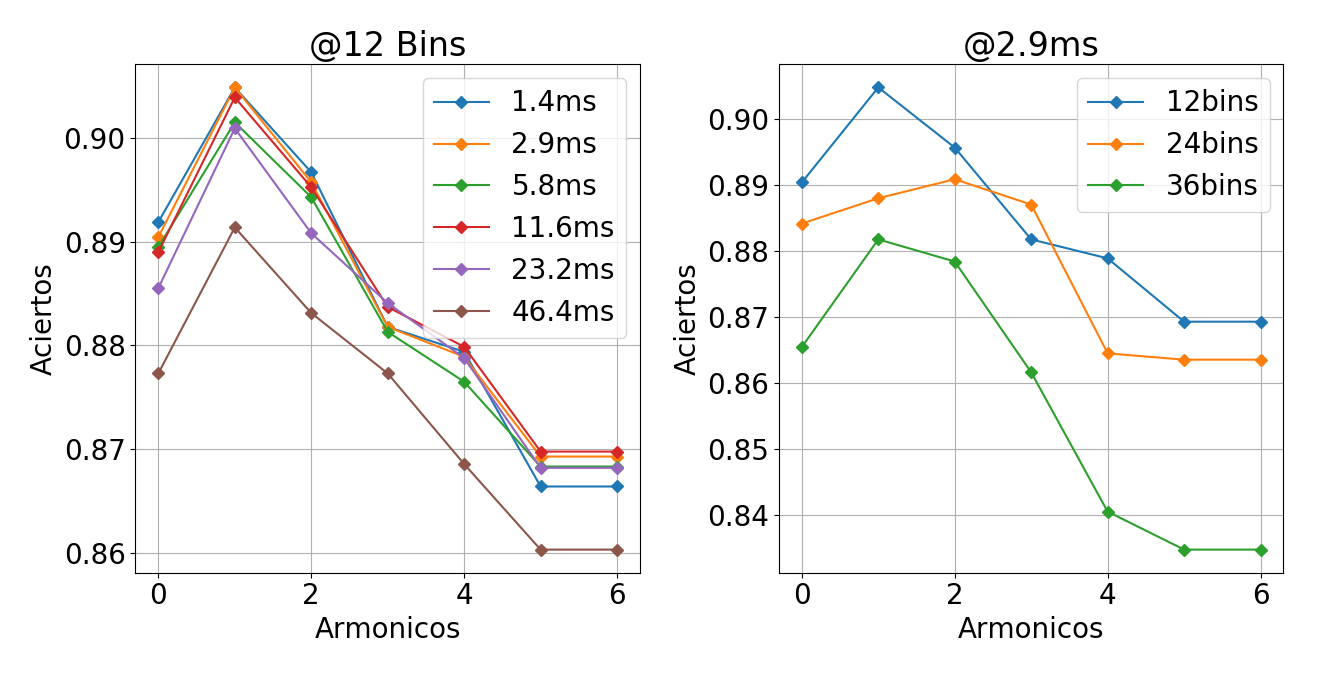
\includegraphics[width=0.5\textwidth]{imagenes/aciertos_cqt} 
\caption{Aciertos en función de la cantidad de armónicos en la codificación, con organización en alturas absolutas. Se observa a la izquierda el ajuste con resolución espectral fija en 12 Bins por octava variando la resolución temporal. A la derecha el ajuste con resolución temporal fija en $2.9ms$ variando la cantidad de bins por octava. }
\label{fig:aciertos_cqt}
\end{center}
\end{figure} 

\begin{figure}[h!]
\begin{center}
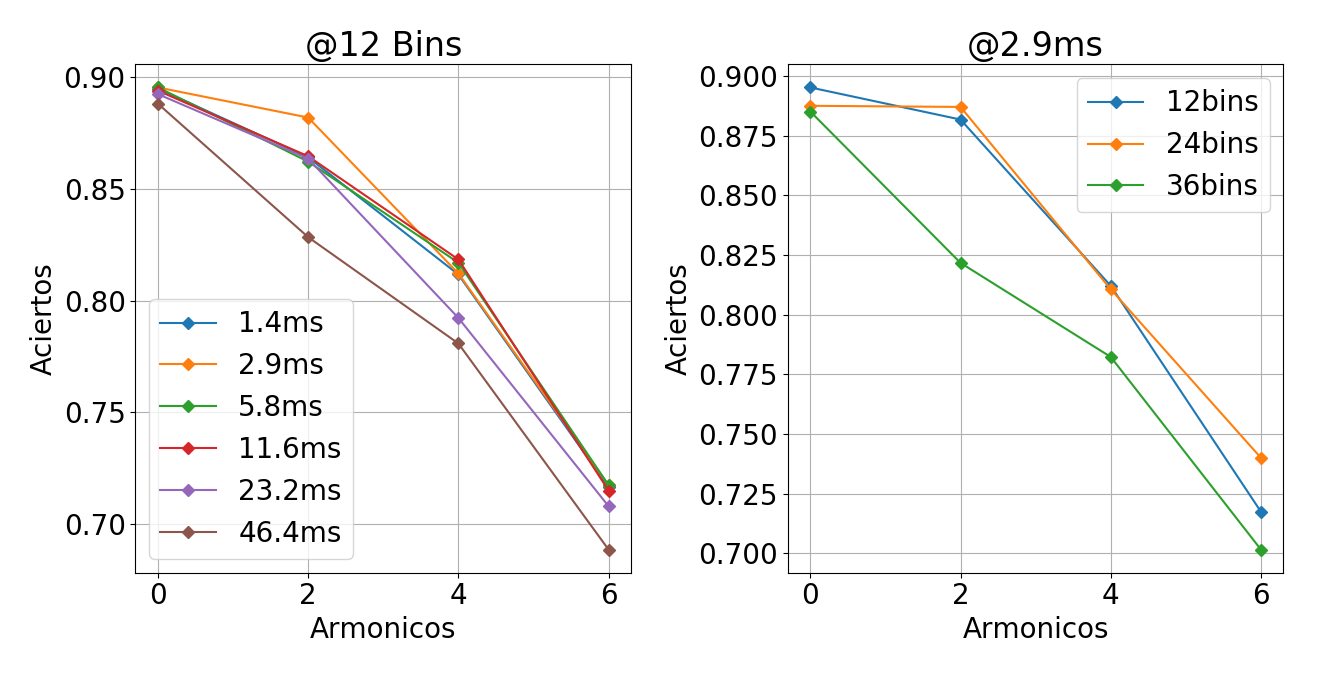
\includegraphics[width=0.5\textwidth]{imagenes/aciertos_chroma} 
\caption{Aciertos en función de la cantidad de armónicos en la codificación, con organización en clase de alturas. Se observa a la izquierda el ajuste con resolución espectral fija en 12 Bins por octava variando la resolución temporal. A la derecha el ajuste con resolución temporal fija en $2.9ms$ variando la cantidad de bins por octava. }
\label{fig:aciertos_chroma}
\end{center}
\end{figure} 

\begin{table}[!ht]
\caption{Tabla con el desempeño en función del parámetro $\beta$.}
\label{tab:beta}
\vspace*{10pt}
\centering
\small
\begin{tabular}{lll}
\textbf{$\beta$}	&	\textbf{Alturas Absolutas} &	\textbf{Clases de Altura}\\ \hline
0.1 & 82\% & 90\% \\
0.4 & 77\% & 87\% \\
0.7 & 76\% & 86\% \\
1.0 & 76\% & 86\% \\
\end{tabular}
\end{table}

\subsection{Comparación}

Vale resaltar que se presentan las estrategias que fueron detalladas a lo largo del presente capítulo, y además se agrega como variante, el cálculo de la matriz de similaridad con distancia euclideana. Para esto se computa la representación intermedia en organización en alturas absolutas con los mejores parámetros de etapa de ajuste (12 bins por octava, $2.9ms$ de resolución temporal y un armónico en la codificación de la partitura). En resumen se hace la comparación de: 

\begin{itemize}

\item \textbf{AA \& Cosine}: Organización en alturas absolutas con los mejores parámetros de la etapa de ajuste (12 bins por octava, $2.9ms$ de resolución temporal y un armónico en la codificación de la partitura) y distancia coseno para el cómputo de la matriz de similaridad.
\item \textbf{AA \& Euclidean}: Organización en alturas absolutas con los mejores parámetros de la etapa de ajuste (12 bins por octava, $2.9ms$ de resolución temporal y un armónico en la codificación de la partitura) y distancia euclideana para el cómputo de la matriz de similaridad.
\item \textbf{CA \& Cosine}: Organización en clases de altura con los mejores parámetros de la etapa de ajuste (12 bins por octava, $2.9ms$ de resolución temporal y un armónico en la codificación de la partitura) y distancia coseno para el cómputo de la matriz de similaridad.
\item \textbf{AA \& Sintesis}: Organización en alturas absolutas y representación intermedia de la notación simbólica realizada mediante la síntesis.  
\item \textbf{CA \& Sintesis}: Organización en clases de altura y representación intermedia de la notación simbólica realizada mediante la síntesis. 

\end{itemize}


\begin{figure}[h!]
\begin{center}
\includegraphics[width=0.5\textwidth]{imagenes/comparacion} 	
\caption{Arriba, tasa de aciertos en función de la tolerancia. Abajo, precisión en forma de \textit{boxplot} para el caso $tol=200ms$. Aclaración: AA refiere a Alturas Absolutas y CA a Clases de Altura.}
\label{fig:comparacion}
\end{center}
\end{figure}

\begin{table}[!ht]
\caption{Tasa de aciertos por obra.}
\label{tab:por_obra}
\vspace*{10pt}
\centering
\small
\begin{tabular}{ll}
\textbf{Obra}	&	\textbf{Resultado}\\ \hline
Allemande     & 96\%   \\
Syrinx & 86\%   \\
Density 21.5 & 80\%   \\
Sequenza I & 70\%   \\
\end{tabular}
\end{table}

Como se observa en la tabla \ref{tab:por_obra}, existe clara superioridad en el movimiento Allemande de BWV 1013 de J.S Bach. Esto es razonable si se tiene en cuenta que es la obra más simple en estructura rítmica. Además, de forma anecdótica sucede que estas medidas se deterioran progresivamente con el momento histórico de cada obra (en orden cronológico: Allemande - Syrinx - Density - Sequenza). La peor tasa de aciertos se da para Sequenza I de L. Berio en correspondencia con su complejidad rítmica.

\section{Conclusiones}

En la tesis aquí descrita se construyó una solución completa al problema de alineación entre audio y partitura para señales de flauta traversa. Para esto, se utilizaron diferentes herramientas de representación tiempo frecuencia y se desarrollaron algoritmos sobre esas representaciones. En adición a lo anterior, se desarrolló una base de datos generada a partir de obras de referencia en el repertorio de la flauta traversa que fue publicada como recurso web con fines académicos.

Por otro lado, se hizo una evaluación objetiva del sistema desarrollado mediante el análisis de la influencia de los distintos parámetros sobre el desempeño final. El análisis tuvo en cuenta además aspectos musicológicos de las obras seleccionadas. Se determinó de esta forma, que el sistema desarrollado es robusto frente a la variación en sus parámetros. Por otro lado, se presentó una comparación final de todas las estrategias implementadas, así como el desempeño de un algoritmo de terceros a modo comparativo. En base a los resultados obtenidos se considera que se resolvió satisfactoriamente el problema planteado inicialmente.

Por último se presentaron los desafíos del repertorio contemporáneo de la flauta traversa para la alineación entre audio y partitura. Además, mediante un caso de estudio se hizo la evaluación de algunas características clásicas en la literatura, para la representación del material sonoro ejecutado con técnicas extendidas.

\subsection{Trabajo a futuro}

Cómo trabajo a futuro queda planteado el uso de DTW en forma online para la implementación de un sistema de acompañamiento automático de flauta traversa con técnicas tradicionales. En cuanto al repertorio contemporáneo el desafío radica en encontrar representaciones matemáticas del material sonoro que puedan ser utilizados como representación intermedia, en sistemas de alineación audio partitura para flauta con técnicas extendidas. 

%%%%%%%%%%%%%%%%%%%%%%%%%%%%%%%%%%%%%%%%%%%%%%%%%%%%%%%%%%%
%
% EJEMPLO DE BIBLIOGRAFÍA
%
% para generar la bibliografía ejecutar "bibtex template"
\bibliographystyle{aes} % estilo aes.bst
\bibliography{bib} % archivo de bibliografía en formato bibtex
%
\end{document} 
